\documentclass[12pt]{article}

\usepackage{graphicx}
\usepackage{float}
\usepackage{amsmath}
\usepackage{amssymb}
\usepackage{graphicx}
\usepackage[utf8]{inputenc}
\usepackage[spanish]{babel}
\usepackage{geometry}
\geometry{left=2cm,right=2cm,top=2cm,bottom=2cm}
\usepackage{listings}
\lstset{basicstyle=\ttfamily,
  showstringspaces=false,
  commentstyle=\color{red},
  keywordstyle=\color{blue}
}


\title{%
  OpenGL\\
  \large Tarea 06 \\
    \Large Computación Gráfica\\
     \large UNAM 2022-2}
\author{Gibran Zazueta Cruz \\
\small 10/mayo/2022}
\date{}

\begin{document}
\maketitle

\section{Introducción}

Se presenta un programa que utiliza las librearías de OpenGL y QT para renderizar un objeto en una ventana. Asimismo, se utiliza la librería de Assimp para cargar un archivo formato Wavefront OBJ. EL objeto a renderizar es el conejo de stanford

En este programa se hace uso de la \textit{Fixed Function Pipeline} de OpenGL, es decir, no se utilizan shaders. La versión de OpenGL utilizada es la 2.1

\section{Escena y materiales}

El objeto cuentan con 2 posibles materiales a seleccionar, estos se definen dentro del código como:

\textbf{Material 1}
\begin{itemize}
\item Ambiental = {0.0, 0.0, 0.0, 1.0},
\item Difusa = {0.50, 0.50, 0.50, 1.0},
\item Especular {0.70, 0.70, 0.70, 1.0} 
\item $\rho$ = 32.0.
\end{itemize}


\textbf{Material 2}
\begin{itemize}
\item Ambiental = {0.23125, 0.23125, 0.23125, 1.0},
\item Difusa = {0.2775, 0.2775, 0.2775, 1.0},
\item Especular {0.773911, 0.773911, 0.773911, 1.0}
\item $\rho$ = 89.6.
\end{itemize}


Se utilizan las texturas

\begin{figure}[H]
\centering

\includegraphics[scale=1]{images/card.jpg}
\caption{Textura material 1}
\end{figure}

\begin{figure}[H]
\centering
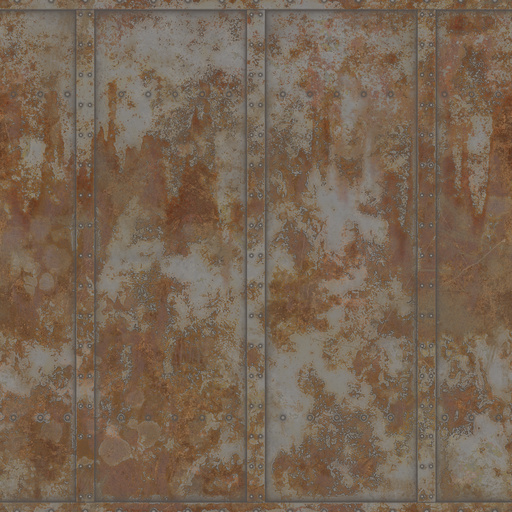
\includegraphics[scale=1]{images/rust.jpg}
\caption{Textura material 2}
\end{figure}



Finalmente, la escena a renderizar cuenta con 2 luces (blanca y azul) y 4 cámaras.

Se disponen de la siguiente manera: 


\begin{figure}[H]
\centering
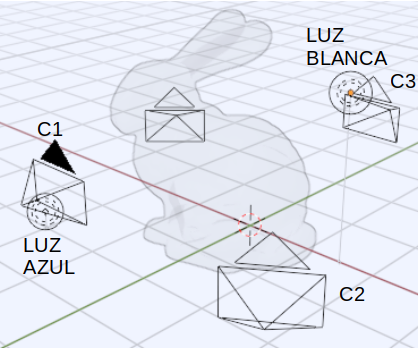
\includegraphics[scale=0.5]{images/escena11.png}
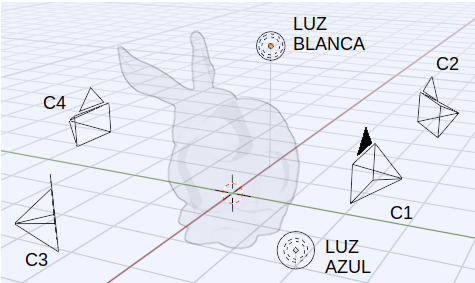
\includegraphics[scale=0.5]{images/escena22.png}
\caption{Posición de las componentes de la escena}
\end{figure}



\section{Estructura del código}

Para almacenar la información del objeto se define la clase \textit{CubeObject} y la  la función \textit{importFile()} que está definida en \textit{functions.cpp}.

Esta función se llama desde \textit{mainwindow.cpp}. La función recibe el path del archivo (como una cadena std::string) y apuntadores al contenedor de vertices, indices de caras, normales y coordenadas de textura del objeto cubeObject, que es el objeto  a renderizar en la escena. Dentro de esta función se utiliza la librería de assimp.

Dentro de mainwindow´ se le dice a qt que utilice OpenGL para dibujar sobre el canvas, esto es con la función \textit{$setSurfaceType(QWindow::OpenGLSurface)$}. También se definen funciones de interacción de ventana como son: \textit{resizeGL}, \textit{initializeGL}, \textit{paintGL}.

Es en \textit{paintGL} donde se dibuja el objeto. Se especifican cámaras, materiales, luces y texturas. Los vértices se definen dentro de un ciclo $for$ para todos los triàngulos del objeto.




\section{Ejecutar el programa}
En la carpeta de build se puede ejecutar el programa con el archivo OpenGLRendering-Run. Desde la consola de comandos de linux:

\begin{lstlisting}[language=bash,title={bash}]
./OpenGLRendering-Run
\end{lstlisting}


En la carpeta principal está el código fuente. Para generar el ejecutable primero se genera el Makefile con

\begin{lstlisting}[language=bash,title={bash}]
 qmake OpenGLRendering.pro
\end{lstlisting}

Después se construye el proyecto con \textit{make}



\section{Instrucciones de uso}


Para cambiar entre las camaras se utilizan las teclas de los numeros
\begin{itemize}
\item "1". Cambia a la cámara 1
\item "2". Cambia a la cámara 2
\item "3". Cambia a la cámara 3
\item "4". Cambia a la cámara 4

\end{itemize}


Para encender y apagar la luz se presiona la tecla \textbf{\textit{6}}. La luz inicia encendida.


Para cambiar entre materiales se utiliza la tecla \textbf{\textit{8}} para el material 1 y la tecla \textbf{\textit{9}} para el material 2.




\section{Programa en ejecución}

\begin{figure}[H]
\centering
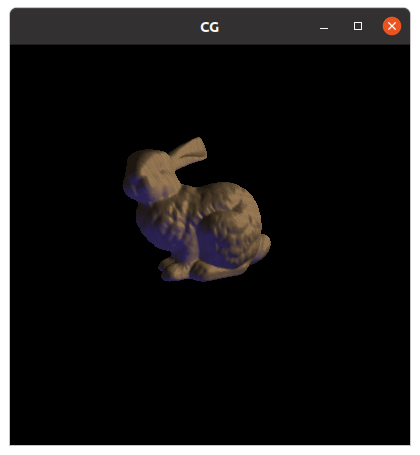
\includegraphics[scale=0.6]{images/ej1.png}
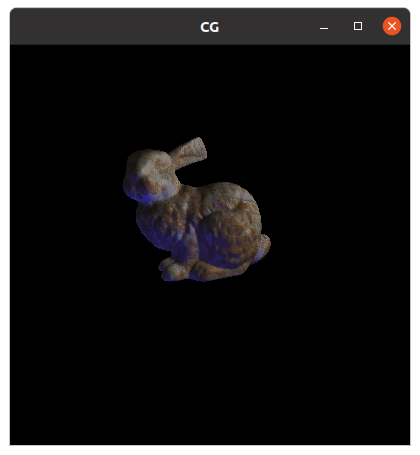
\includegraphics[scale=0.6]{images/ej2.png}
\caption{Renderizado cámara 1, materiales 1 y 2}
\end{figure}

\begin{figure}[H]
\centering
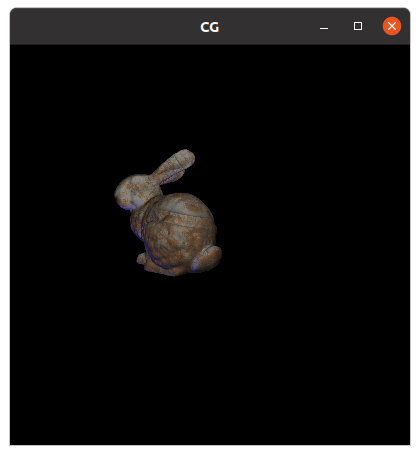
\includegraphics[scale=0.4]{images/ej3.png}
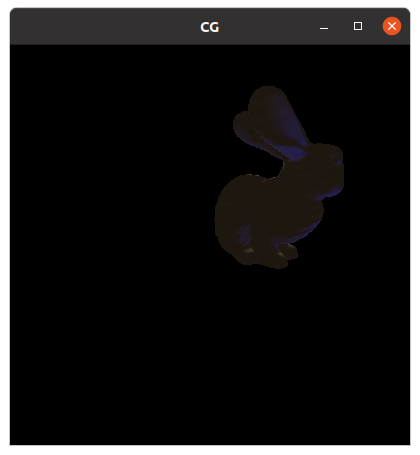
\includegraphics[scale=0.4]{images/ej5.png}
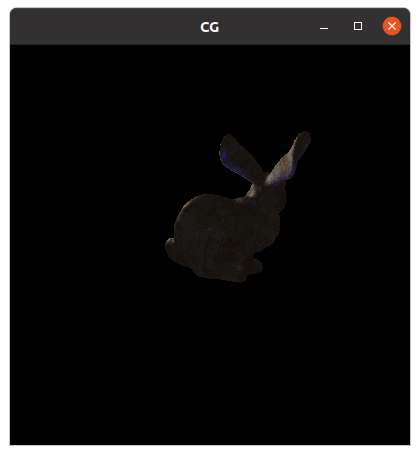
\includegraphics[scale=0.4]{images/ej4.png}
\caption{Renderizado cámara 2, 3 y 4. Material 2}
\end{figure}


%\begin{thebibliography}{99}


%\bibitem{open} Wavefront obj file. ($https://en.wikipedia.org/wiki/Wavefront_.obj_file$)

%\end{thebibliography}


\end{document}
